

%%%%\section{Mu3e}

The $\mu \rightarrow eee$ decay is a charged lepton flavor violating process strongly suppressed in the 
Standard Model. New physics mediated either via virtual loop or three diagrams can enhance these rates 
to values accessible by the next generation of experiments. An interesting feature of this process is 
the possibility to determine the chirality of New Physics, should it be observed with sufficient 
statistics~\cite{Okada:1999zk}. We present a study to search for $\mu \rightarrow eee$ decay using the FastSim 
simulation package. The experimental setup, inspired from the Mu3e experiment~\cite{Blondel:2013ia}, is a compact 
tracker surrounding a target formed by two hollow cones. The tracker consists of 6 layers of 
cylindrical silicon detectors, each composed of 50 $\mu$m thick silicon sensors mounted on 
50 $\mu$m of kapton. The cones forming the target have a length and diameter of 5 cm and 1 cm, 
respectively. Contrary to Mu3e, we consider an active target made of silicon pixel detectors, 
assuming a pixel size of 50 $\mu$m by 50 $\mu$m. Although not included, a time-of-flight system 
should be installed as well, providing a time measurement with a resolution between 50 - 500 ps. 
The full apparatus is displayed in Fig.~\ref{Fig::mu3e}, together with a simulated 
$\mu^+ \rightarrow e^+e^-e^+$ event.

We generate $\mu^+ \rightarrow e^+e^-e^+$ events according to phase space, and reconstruct the 
decays constraining the tracks to originate from the same position on the target. The vertex 
position is chosen by considering all points from tracks intercepting the target, and 
choosing the one minimizing the $\chi^2$ of the constrained fit. To further improve the 
resolution, we require the probability of the constrained fit to be greater than 1\%, and a 
reconstructed muon momentum less than $1 ~\Mev$. The resulting $e^+e^-e^+$ invariant mass 
distribution, shown in Fig.~\ref{Fig::mu3e}, is fitted with a sum of two Gaussian functions. A 
core (tail) resolution of 0.3 (0.8)~\Mev\ is observed for a signal efficiency of 12\%. 

To achieve a single event sensitivity at the level of $\sim 10^{-17}$ after a 1-year run, 
a rate of stopped muons in the target of the order of $3 \times 10^{10}$ is needed, assuming 
a reconstruction efficiency of $\sim10\%$. For the purpose of estimating background 
contributions, we define a signal window as $ 104.8 < m_{eee} < 107.3 ~\Mev$, containing 
approximately 90\% of the signal. 

The accidental background arise from $\mu \rightarrow e^+e^-e^+ \nu\nu$ events where the two 
neutrinos carry almost no energy. We estimate its contribution to be about 3 events by 
convolving the branching fraction with the resolution function and integrating in the 
signal region. An efficiency of 10\% is assumed. One must note that this background depends 
strongly on the tail resolution, and a small improvement translates into a large decrease 
of this contamination. For example, reducing the tail resolution to 0.5~\Mev\ decreases 
this contamination to $\sim 0.5$ event. Simulation indicate that such a resolution could be 
achieved for silicon sensors 50\% thinner.

We consider accidental backgrounds produced by the combination of a Michel decay and a radiative Michel 
decay (2M$\gamma$ decays), or three simultaneous Michel decays (3M decays), where one the the positron 
is misreconstructed or produce an electron by interacting with the detector. In both cases, we assume 
the decays occurs within the same pixel in the active target and within the same time widow, taken to 
be 250 ps. This yields position and time suppression factors $\delta S = 7.8\times 10^{-7}$ and 
$\delta t = 2.5\times 10^{10}$, respectively. The expected number of background events is:
%
$$N_{2M\gamma} = R^2 \delta S \delta t BF(\mu^+ \rightarrow e^+ \nu_e \bar\nu_\mu \gamma) P(\gamma \rightarrow e^+ e^-) P_\mu  \sim 5\times 10^7 P_\mu$$
$$N_{3M} = R^3(\delta S)^2 (\delta t)^2 P_\mu \sim 3 \times 10^7 P_\mu$$
%
where $P(\gamma \rightarrow e^+ e^-)$ is the probability of photon conversion and $P_\mu$ denotes the 
probability to reconstruct a muon candidate after all selection criteria are applied. Considering only 
photon conversion in the target, the probability $P(\gamma \rightarrow e^+ e^-) \sim 0.001$. The factors 
$P_\mu$ need therefore to be at least of the order of $10^{-8}$ to limit the background to fraction of 
event.

The advantage of the active target w.r.t. the Mu3e design is essentially in the reduction of the accidental 
background rate, while slight improvements in the resolution should reduce the $\mu \rightarrow e^+e^-e^+ \nu\nu$ 
contamination at appropriate levels. 

\begin{figure}[htb]
\begin{center}
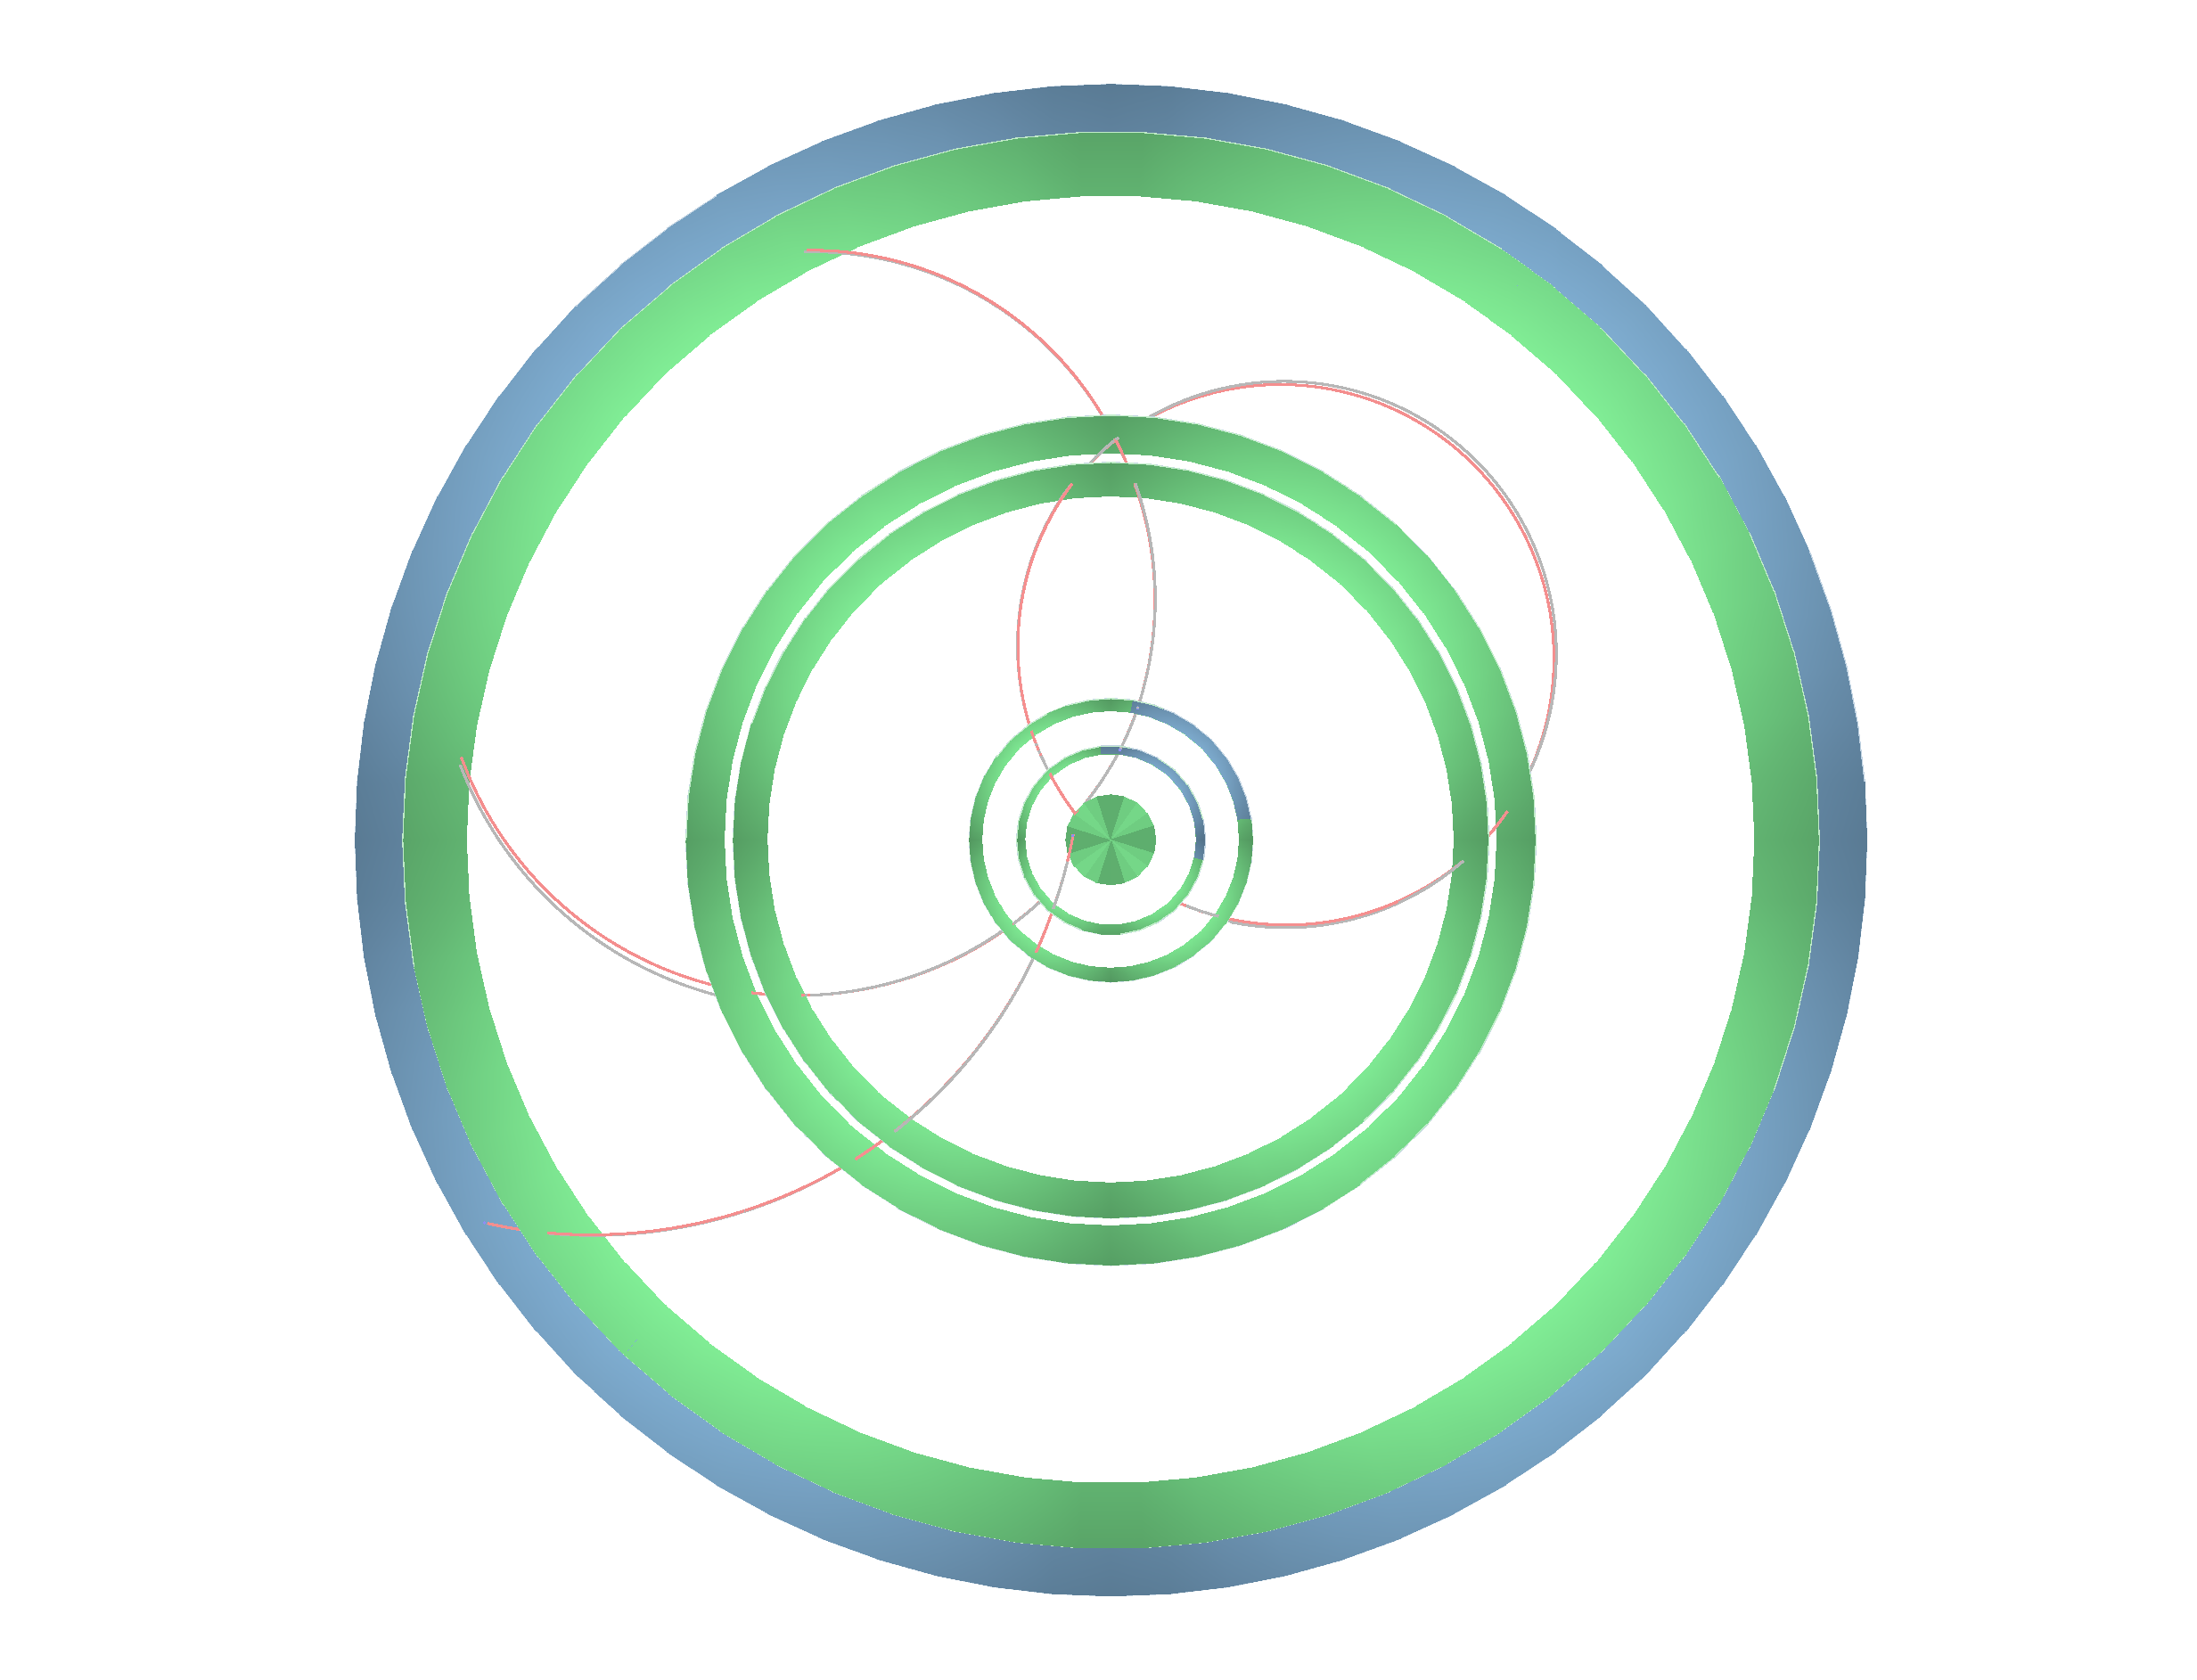
\includegraphics[width=0.45\textwidth]{ChargedLeptons/Figures/event.pdf}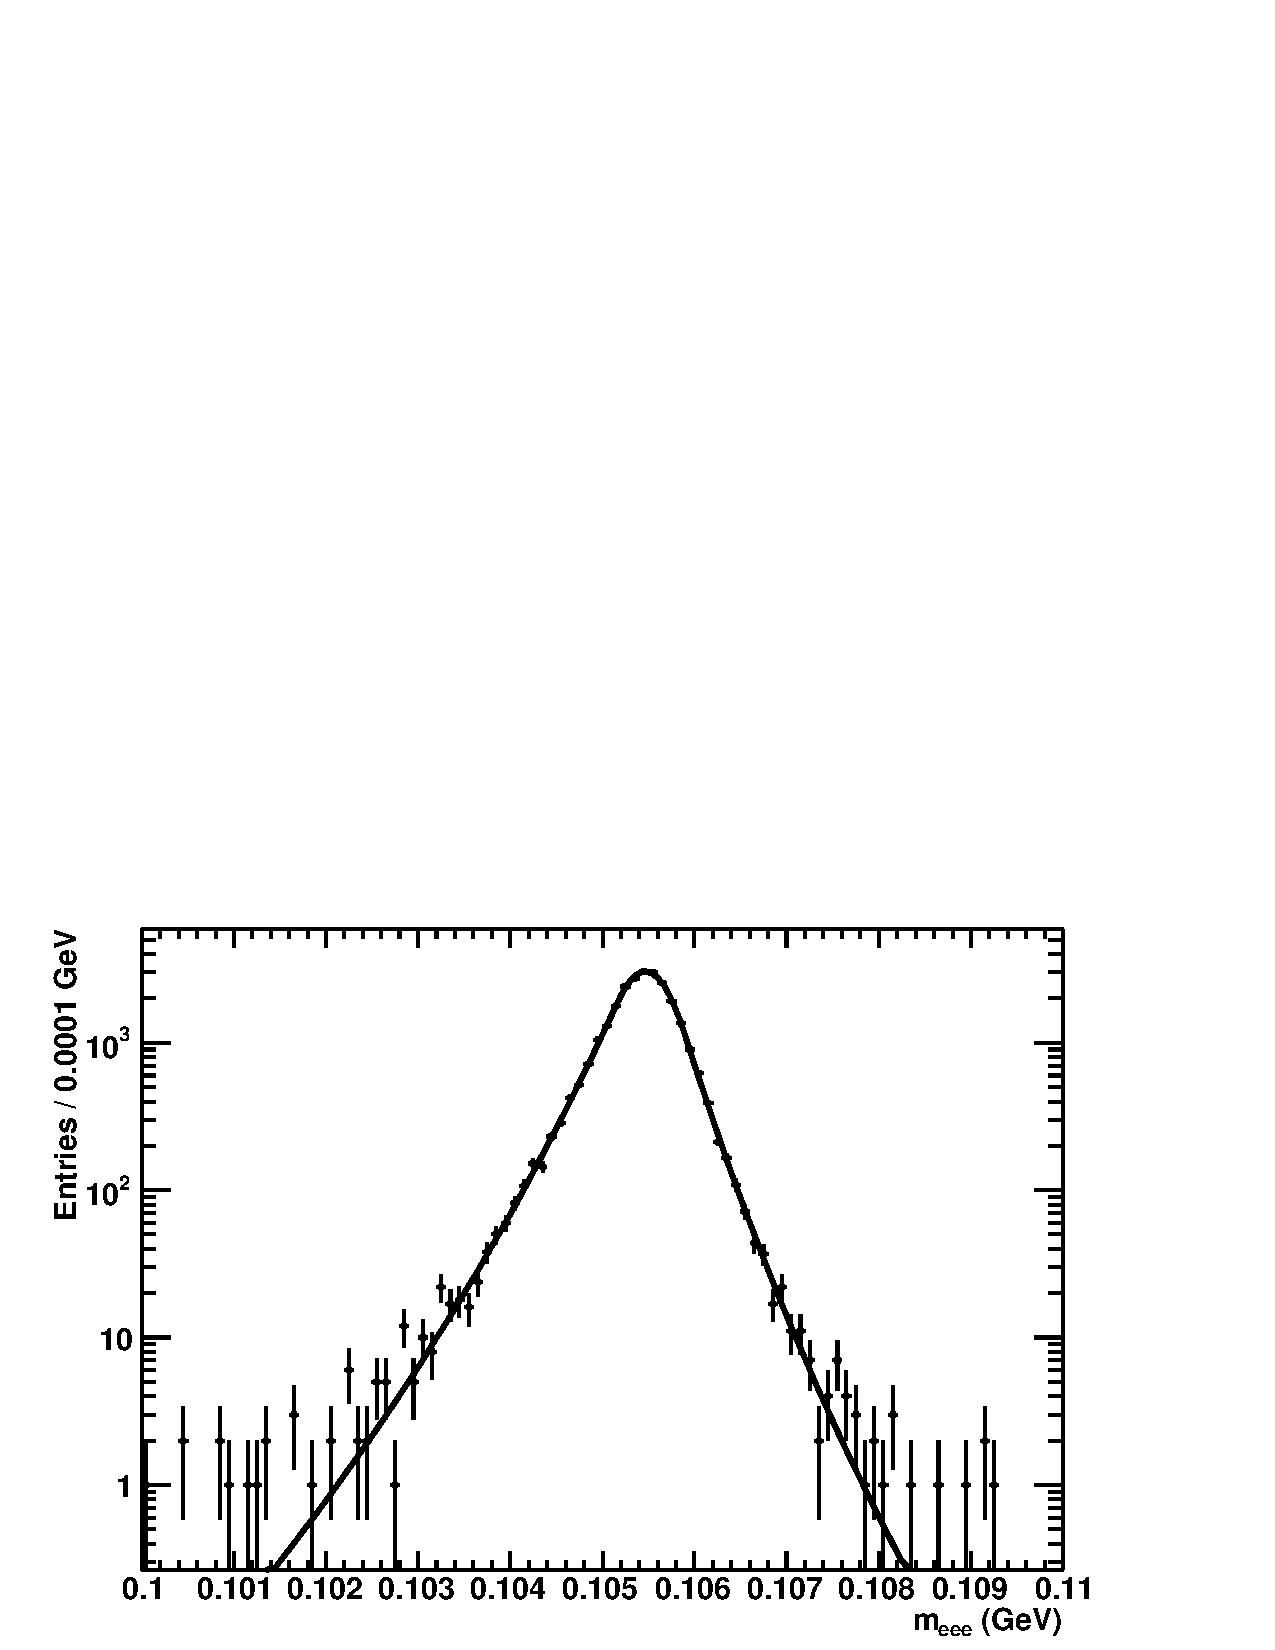
\includegraphics[width=0.45\textwidth]{ChargedLeptons/Figures/resoFit.pdf}
\end{center}
\caption
{Left: Display of the experimental setup, together with a simulated $\mu^+ \rightarrow e^+e^-e^+$ event. 
Right:  The $e^+e^-e^+$ invariant mass distribution after all selection criteria are applied fitted by a 
sum of two Gaussian functions.}
\label{Fig::mu3e}
\end{figure}




